\documentclass{beamer}
\usepackage{graphicx}
\usepackage{paralist}
\usepackage{outlines}

\title{Image Adjustment Tools}
\author{Mendocino College - Digital Image Manipulation with Photoshop}
\titlegraphic{\vspace{-10mm}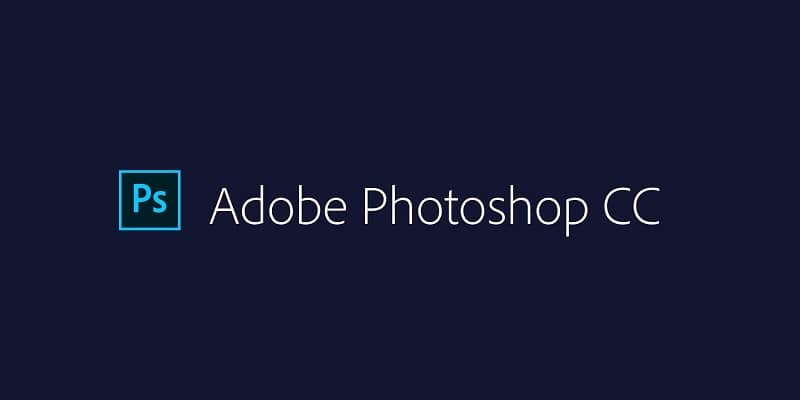
\includegraphics[width = .9\textwidth]{images/photoshop.jpg}} 
\date{\vspace{-5em}} 


\mode <presentation>
\usetheme{Warsaw}
\usecolortheme{default}

\setbeamerfont{footline}{size=\fontsize{5}{8}\selectfont}

\definecolor{darkred}{rgb}{20,0,0}
\definecolor{darkgreen}{RGB}{40,110,20}
\definecolor{darkpurple}{RGB}{30,0,30}
\definecolor{chardonnay}{RGB}{255, 255, 204}

\setbeamercolor*{palette primary}{fg=white, bg=darkgreen}


\begin{document}
	{
		\setbeamertemplate{footline}{} 
		\setbeamertemplate{headline}{} 
		\begin{frame}
			\vspace{-35pt}
			\maketitle
		\end{frame}
	}


		\section{Blur and Sharpen Tools}
			\subsection{Blur Tool}		
			\begin{frame}
				\frametitle{Blur Tool}
				\begin{outline}
					\1 The Blur tool softens hard edges or reduces detail in an image.
					\1 It allows you to paint the blur effect on specific areas of an image.
					\1 The more you paint over an area with the tool, the blurrier it becomes.
					\1 Select the Blur tool, and drag over the part of the image you want to blur.
				\end{outline}
							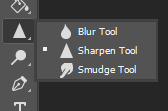
\includegraphics[width=0.5\textwidth]{images/sharpen tool.png}
			\end{frame}
		
					\subsection{Blur Tool Example}		
		\begin{frame}
			\frametitle{Blur Tool Example}
			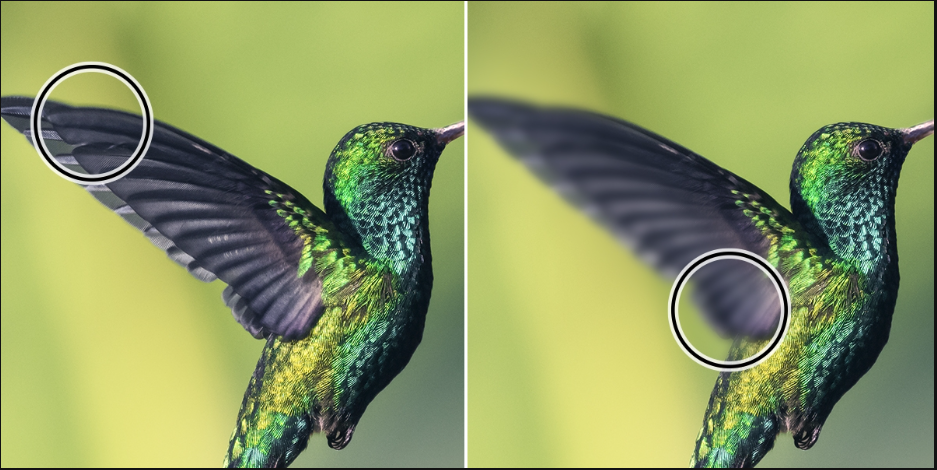
\includegraphics[width=1.0\textwidth]{images/blur tool.png}
		\end{frame}

			\subsection{Sharpen Tool}		
	\begin{frame}
		\frametitle{Sharpen Tool}
				\begin{outline}
					\1 The Sharpen tool increases contrast along edges to increase apparent sharpness. 
					\1 It allows you to paint the sharpen effect on specific areas of an image.
					\1 The more you paint over an area with the tool, the more sharpening increases.
					\1 Select Protect Detail to enhance details and minimize pixelated artifacts. 
					\2 Deselect this option if you want to produce more exaggerated sharpening effects.
				\end{outline}
		\end{frame}
	
				\subsection{Sharpen Tool Example}		
	\begin{frame}
		\frametitle{Sharpen Tool Example}

		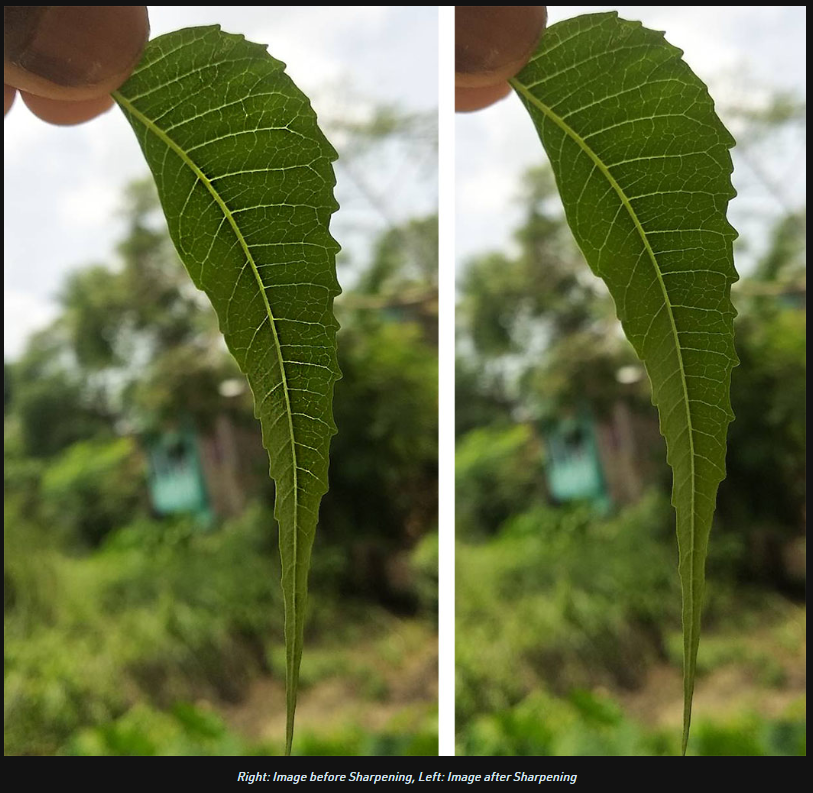
\includegraphics[width=0.7\textwidth]{images/sharpen tool example.png}
	\end{frame}
			
		\section{Smudge Tool}
			\subsection{Smudge Tool}		
			\begin{frame}
				\frametitle{Smudge Tool}
				\begin{outline}
					\1 The Smudge Tool smooths and blends colors.
					\1 It simulates the effect of dragging a finger through wet paint.
					\1 The tool picks up color where the stroke begins and pushes it in the direction you drag.
					\1 Select Finger Painting in the options bar to smudge using the foreground color at the beginning of each stroke. 
					\2 Deselect Finger Painting to use the color under the pointer at the beginning of each stroke.
					\2 Press Alt (Windows) or Option (Mac OS) as you drag with the Smudge tool to use the Finger Painting option.
					\2 Deselect this option if you want to produce more exaggerated sharpening effects.
				\end{outline}
			\end{frame}
		
		\subsection{Smudge Tool Example}		
		\begin{frame}
			\frametitle{Smudge Tool Example}
			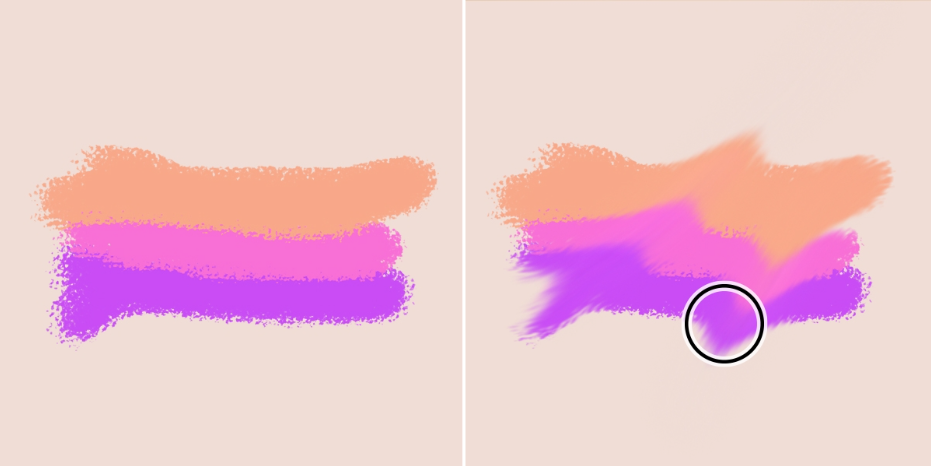
\includegraphics[width=1.0\textwidth]{images/smudge tool.png}
		\end{frame}
			
		\section{Dodge and Burn Tools}
			\subsection{Dodge Tool}		
			\begin{frame}
				\frametitle{Dodge Tool}
								\begin{outline}
					\1 The Dodge tool allows you to lighten specific areas of your image without affecting hue or saturation.
					\1 These tools are based on a traditional darkroom technique for regulating exposure on specific areas of a print.
					\1 Photographers hold back light to lighten an area on the print (dodging) or increase the exposure to darken areas on a print (burning). 
					\1 The more you paint over an area with the Dodge tool, the lighter it becomes.
				\end{outline}
			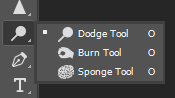
\includegraphics[width=0.5\textwidth]{images/doge and burn tools.png}
			\end{frame}
		
					\subsection{Dodge Tool Example}		
		\begin{frame}
			\frametitle{Dodge Tool Example}
			\includegraphics[width=1.0\textwidth]{images/dodge tool.png}
		\end{frame}
		
		\subsection{Burn Tool}		
			\begin{frame}
				\frametitle{Burn Tool}
				\begin{outline}
					\1 The Burn tool selectively darkens an area in your image.
					\1 The options bar has the following options:
					\2 Midtones   - Changes the middle range of grays
					\2 Shadows    - Changes the dark areas
					\2 Highlights - Changes the light areas
					\2 Exposure   - Sets the amount of light for the stroke.
					\2 Airbrush   - Switches between Brush and Airbrush.
					\2 Protect Tones -  Minimize clipping in the shadows and highlights. It also tries to keep colors from shifting hue.
				\end{outline}
			\end{frame}
		
		\subsection{Burn Tool Example}		
			\begin{frame}
				\frametitle{Burn Tool Example}
				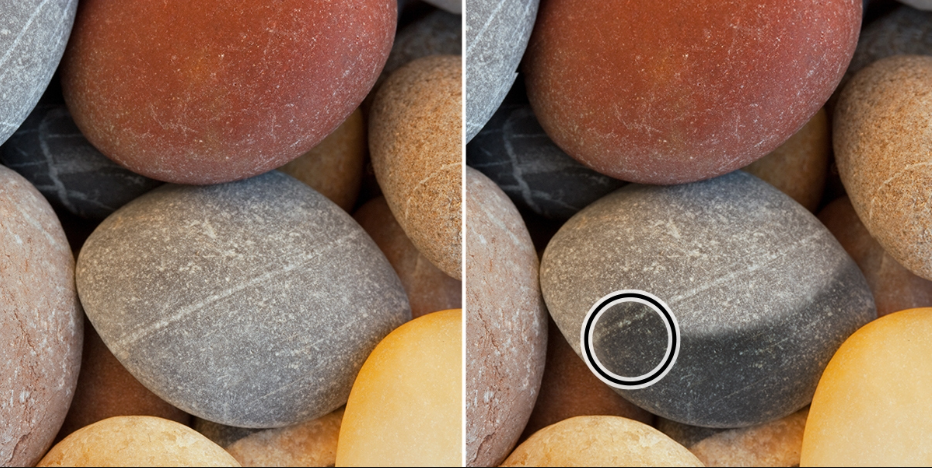
\includegraphics[width=1.0\textwidth]{images/burn tool example.png}
			\end{frame}
	
		\section{Sponge Tool}
			\subsection{Sponge Tool}		
				\begin{frame}
					\frametitle{Sponge Tool}
					\begin{outline}
						\1 Use the Sponge tool to change color saturation of areas in an image.
						\1 The Sponge tool subtly changes the color saturation of an area.
						\1 When an image is in Grayscale mode, the tool increases or decreases contrast by moving gray levels away from or toward the middle gray.
						\1 The options bar has the following options:
						\2 Brush tip and set brush options.
						\2 Mode - 
						\3 Saturate: Intensifies the color's saturation.
						\3 Desaturate:  Dilutes the color's saturation.
						\2 Flow - sets the rate of saturation change.
						\2 Vibrance - to minimize clipping for fully saturated or desaturated colors.
					\end{outline}
				\end{frame}
			
			\subsection{Sponge Tool Example}		
	\begin{frame}
		\frametitle{Sponge Tool Example}
		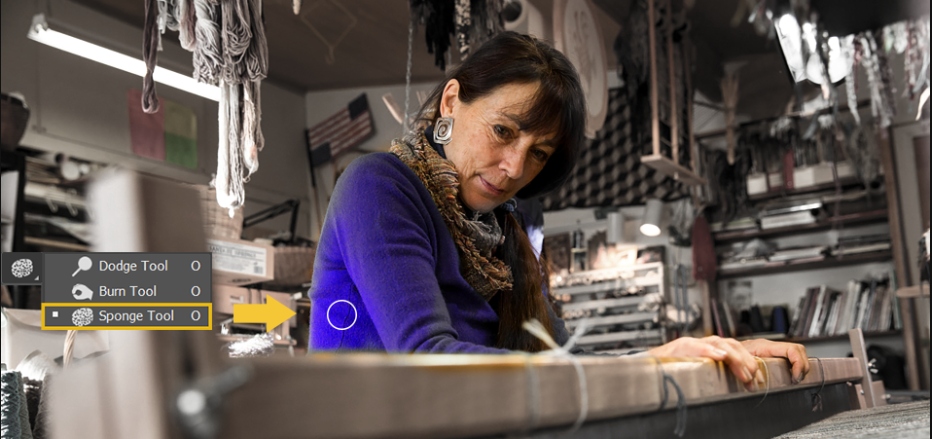
\includegraphics[width=1.0\textwidth]{images/sponge tool example.png}
	\end{frame}

		\section{}
			\subsection{Destructive Edits}		
			\begin{frame}
				\frametitle{Destructive Edits}
				\begin{outline}
					\1 Applying these tools permanently alters the image information.
					\1 It is recommended to always work using nondestructive edits.
					\1 To edit your images nondestructively, work on a duplicate layer. 
				\end{outline}
				\begin{center}
					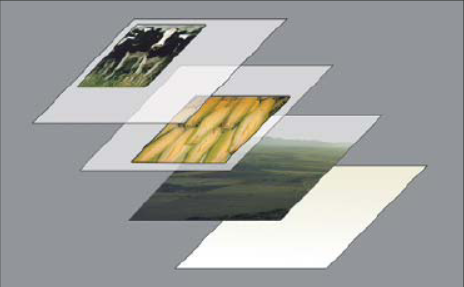
\includegraphics[width=0.7\textwidth]{images/layers example.png}
				\end{center}	
			\end{frame}
	
\end{document}